% Author: David Larsen <dcl9934@cs.rit.edu>
% Author: Doug Krofcheck <dpk3062@rit.edu>
\documentclass[11pt]{article}
\usepackage[margin=0.7in]{geometry}
\usepackage{listings}   %
\usepackage{needspace}  %
\usepackage{color}      %
\usepackage{ifthen}     % 
\usepackage{graphicx}   %
\usepackage{csc}        %
\usepackage{tikz}       %
\usetikzlibrary{shapes, arrows, automata} %
\usepackage{tabularx}   % for helping matchtabular (matching questions)
\usepackage{textcomp}	% So our quotes in code don't look like shit
\usepackage{longtable}
\usepackage{multicol}
\setlength{\columnsep}{12em}

\lstset{ %
basicstyle=\footnotesize\ttfamily,       % the size of the fonts that are used for the code
numbers=left,                   % where to put the line-numbers
stepnumber=1,                   % the step between two line-numbers. If it's 1 each line will be numbered
numbersep=5pt,                  % how far the line-numbers are from the code
showspaces=false,               % show spaces adding particular underscores
showstringspaces=false,         % underline spaces within strings
tabsize=4,		                % sets default tabsize to 4 spaces
language=Java,
upquote=true,
columns=fixed
}

\ifthenelse{\isundefined{\isAnswerKey}}
{
    \newenvironment{answer}{\large\lstset{basicstyle=\large\ttfamily}\color{white} \small{Answer:}}{}
}
{
    \newenvironment{answer}{\large\lstset{basicstyle=\large\ttfamily}\color{red} \small{Answer:}}{}
}

% ----- Start matchtabular definition -----
\newcounter{matchleft}
\newcounter{matchright}
\newenvironment{matchtabular}{%
  \setcounter{matchleft}{0}%
  \setcounter{matchright}{0}%
  \tabularx{\textwidth}{%
    >{\leavevmode\hbox to 1.5em{\stepcounter{matchleft}\arabic{matchleft}.}}X%
    >{\leavevmode\hbox to 1.5em{\stepcounter{matchright}\alph{matchright})}}X% 
    }%
}{\endtabularx}
% ----- End matchtabular definition -----

\title{CSCI-142 Exam 2 Review}
\author{Computer Science Community}
\date{\today}

\makeatletter
\let\thetitle\@title
\let\theauthor\@author
\let\thedate\@date
\makeatother

\begin{document}
\header
\begin{enumerate}


\item Suppose we are talking about the depth-first search (DFS) algorithm.
Assume nodes are \emph{added} to the data structure in alphabetical order.
\begin{enumerate}
\item What underlying data structure does this algorithm use?

\begin{answer}
A stack.
\end{answer}

\item %b
Given the following graph, state the path that the DFS would generate and show the data structure at each step.
Node \texttt{A} is the start node, and \texttt{F} is the desination node.

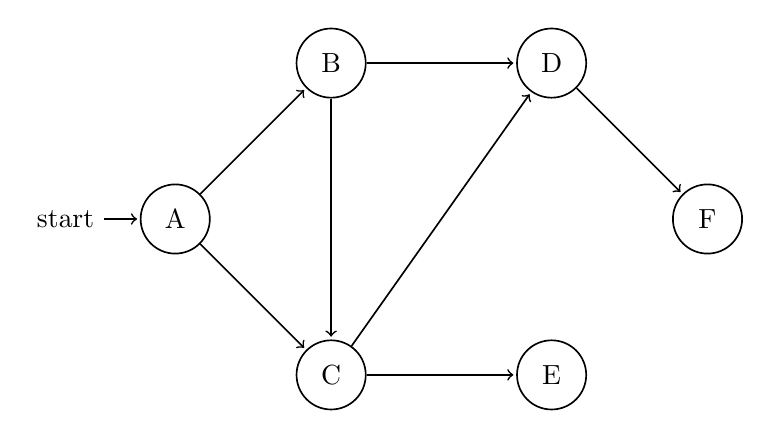
\begin{tikzpicture}[shorten >=1pt,auto,node distance=2.8cm,semithick]
	\node[initial,state] (A) {A};
	\node[state]        (B) [above right of=A] {B};
	\node[state]        (C) [below right of=A] {C};
	\node[state]        (D) [right of=B] {D};
	\node[state]        (E) [right of=C] {E};
	\node[state]        (F) [below right of=D] {F};

	\path[->]   (A) edge node {} (C)
		(A) edge node {} (B)
		(B) edge node {} (C)
		(B) edge node {} (D)
		(C) edge node {} (D)
		(C) edge node {} (E)
		(D) edge node {} (F);
			
\end{tikzpicture}

\begin{answer}
The traversal order is ACEDF.
\end{answer}

\item %c
What changes would we need to implement to make use of a breadth-first search (BFS) algorithm?

\begin{answer}
Use a queue data structure (instead of a stack.)
\end{answer}

\end{enumerate}

\item Question \\
\begin{answer}
Answer
\end{answer}


\item Question \\
\begin{answer}
Answer
\end{answer}



\item Is there anything wrong with the following exception handler as written? Will this
code compile? 
\begin{lstlisting}[language=java]
try {
this.epicFail();
} catch (Exception e) {
} catch (ArithmeticException a) {
}
\end{lstlisting}
\begin{answer}
\\ In Java 6: No problem :)
\\ In Java 7: Compile error!  Exception is more generic than ArithmeticException so the second catch statement is unreachable.
\end{answer}



\item Write code to naturally sort the given list in as few lines as possible. You'll lose half
of the points if you use a loop. Do not use any numbers (Integers, ints, Double, double,
BigInteger, etc...).
\begin{lstlisting}[language=java]
List<String> list = Arrays.asList("a", "o", "d", f", "x");
\end{lstlisting}
\begin{answer}
\\Collections.sort(list);
\\//or
\\TreeSet<String> sorted = new TreeSet<String>(list);
\end{answer}


\newpage
\item Describe each of the following layout managers:
\begin{enumerate}
\item FlowLayout
\begin{answer}
The FlowLayout class puts components in a row, sized at their preferred size. If the horizontal space in the container is too small to put all the components in one row, the FlowLayout class uses multiple rows. If the container is wider than necessary for a row of components, the row is, by default, centered horizontally within the container. To specify that the row is to aligned either to the left or right, use a FlowLayout constructor that takes an alignment argument. Another constructor of the FlowLayout class specifies how much vertical or horizontal padding is put around the components. \end{answer}
\item BorderLayout
\begin{answer}
With a Boarder layout, if the window is enlarged, the center area gets as much of the available space as possible. The other areas expand only as much as necessary to fill all available space. Often a container uses only one or two of the areas of the BorderLayout object — just the center, or the center and the bottom. \end{answer}
\item GridLayout
\begin{answer}
A GridLayout object places components in a grid of cells. Each component takes all the available space within its cell, and each cell is exactly the same size. If the GridLayoutDemo window is resized, the GridLayout object changes the cell size so that the cells are as large as possible, given the space available to the container.\end{answer}
\end{enumerate}




\item Discuss the differences between ArrayList and LinkedList. Which list should you prefer in the following situations:
\begin{enumerate}
\item Inserting a random number into a sorted list.
\item Creating a list that will hold all the players in a game.  The game has a max limit on the amount of players.  
\item Deleting from near the tail end of the list.
\item Deleting from the head end of the list.
\end{enumerate}
\begin{answer}
LinkedList is implemented as a doubly-linked list.
\\ArrayList is implemented as a dynamically resizing array.
\\ \\ArrayList allows fast random access, but adding or remove from the middle of the array
requires shifting all the elements. LinkedList always has constant-time insertions or removals
if accessed through an iterator (thus we already know the insertion/removal point), but getting
an element requires traversing the list until we get to the wanted index.
\\ \\ArrayLists take up a specific block of sequential memory. If the list isn't full the extra
memory will be wasted. LinkedList take up random segments of memory and require
forward and backward pointers for each element, but all of it's allocated memory is used.
\begin{enumerate}
\item LinkedList - Constant insertion time (ArrayList will have to adjust index values of all elements after the insertion point).
\item ArrayList - You have a fixed limit, so pre-allocate enough space for that amount.
\item ArrayList - Your linked list may have to iterate all the way down, while the ArrayList just jumps to the right spot.
\item LinkedList - Constant time operation, but O(n) for the ArrayList.
\end{enumerate}
\end{answer}


\newpage
\item Create a class that constructs and displays the following GUI.  The main buttons don't need to do anything when clicked, but the title bar buttons should function as expected (minimize, maximize, exit).  You may or may not need the following: JTextField, JButton, BorderLayout, BoxLayout, FlowLayout.LEFT, JFrame, thousands of dollars, JFileChooser, JComponent, JDesktopPane, and an exit on close operation.  The window is 300 by 300 pixels and has a title.  If you're a board, make the Clear button's text red.
\begin{center}
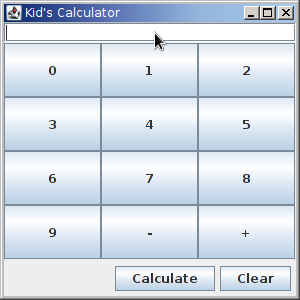
\includegraphics[scale=0.6]{calculator.png}
\end{center}
\begin{answer}
\begin{lstlisting}[language=java]
import java.awt.BorderLayout; import java.awt.Color;
import java.awt.Container; import java.awt.FlowLayout;
import java.awt.GridLayout;

import javax.swing.BoxLayout; import javax.swing.JButton;
import javax.swing.JFrame; import javax.swing.JPanel;
import javax.swing.JTextField;

public class BasicGUI {

	public BasicGUI() {
		JFrame frame = new JFrame("Kid's Calculator");
		frame.setLayout(new BorderLayout());
		
		JPanel top = new JPanel();
		top.setLayout(new BoxLayout(top, BoxLayout.LINE_AXIS));
		top.add(new JTextField());
		
		JPanel center = new JPanel();
		center.setLayout(new GridLayout(4,3));
		for(int i = 0; i < 10; ++i) {
			center.add(new JButton(Integer.toString(i)));
		}
		center.add(new JButton("-"));
		center.add(new JButton("+"));
		
		JPanel bottom = new JPanel();
		bottom.setLayout(new FlowLayout(FlowLayout.RIGHT));
		bottom.add(new JButton("Calculate"));
		JButton clearButton = new JButton("Clear");
		clearButton.setForeground(Color.red);
		bottom.add(clearButton);
		
		Container pane = frame.getContentPane();
		pane.add(top, BorderLayout.NORTH);
		pane.add(center, BorderLayout.CENTER);
		pane.add(bottom, BorderLayout.SOUTH);
		
		frame.pack();
		frame.setSize(300, 300);
		frame.setDefaultCloseOperation(JFrame.EXIT_ON_CLOSE);
		frame.setVisible(true);
	}
	
	public static void main(String[] args) {
		BasicGUI gui = new BasicGUI();
	}
}
\end{lstlisting}
\end{answer}



\item Briefly explain the differences between the three kinds of exceptions: checked exceptions, runtime exceptions, and errors.
\begin{answer}
\textbf{checked exceptions} -– Exceptions that a method signature must specify it throws. If a method
may throw a checked exception then calls to that method must be within a try-catch block. It
is generally assumed that checked exception represent minor issues and any reasonably robust
system should be able to recover from a checked exception. Classic example is IOException.\\

\textbf{runtime exception} -– Not declared in a method signature and not anticipated to be thrown.
Usually represents a major software issue and often causes the program to crash. Classic
examples are NullPointerException and ArrayIndexOutOfBoundsException.\\

\textbf{errors} -– Represent a serious issue outside of the control of the programmer (hard drive
failure, not enough memory, device issue). Examples are IOError, VirtualMachineError and
ThreadDeath (see java's Error class).
\end{answer}



\item Given the following code snippet, rewrite ControlListener as an anonymous class passed into the addActionListener method calls.  
\begin{lstlisting}[language=java]
class ControlListener implements ActionListener{
	public void actionPerformed(ActionEvent e) {
		if((JButton)e.getSource()).getText().equals("ok")) {
			System.exit(0);
		} else {
			log.debug("User pressed cancel.");
		}
	}
}

ControlListener cListener = new ControlListener();
JButton okButton = new JButton("ok");
JButton cancelButton = new JButton("cancel");
okButton.addActionListener(cListener);
cancelButton.addActionListener(cListener);
\end{lstlisting}
\begin{answer}
\begin{lstlisting}[language=java]
JButton okButton = new JButton("ok");
okButton.addActionListener(new ActionListener() {
	public void actionPerformed(ActionEvent e) {
		System.exit(0);
	}
});

JButton cancelButton = new JButton("cancel");
cancelButton.addActionListener(new ActionListener() {
	public void actionPerformed(ActionEvent e) {
		log.debug("User pressed cancel.");
	}
});
\end{lstlisting}
\end{answer}












\end{enumerate}
\end{document}

Topics for this exam:
	- Graphs: DFS/BFS
		#s
	- Dijkstra's Shortest Path
		#s
	- Java Collection Framework, Iterators, Comparators
		#s
	- Intro. to GUIs (from OO perspective)
		#s
	- Swing
		#s
	- Exceptions
		#s

1) brief description of ?
2) 
3) 
4) 
6) 
7) 
8) 
9) 
